    \chapter{Création, récupération et intégration des données}

Les données sont rarement homogènes ou immobiles\footnote{Les données tendent toujours à évoluer dans le temps, que ce soit par l’ajout de métadonnées par exemple, ou de format etc…} : elles peuvent nous parvenir dans différents formats et sont parfois incomplètes, elles peuvent également s’avérer difficiles à récupérer. Cela met en évidence plusieurs enjeux à examiner :  l’ accès aux données, la pluralité des  formats et la fraîcheur de  ces données (sont-elles complètes, y aura-t-il des mises à jour ?).


    \section{Accès aux données}

La première étape est de pouvoir tout simplement accéder à ces données. En reprenant les exemples des projets mentionnés précédemment, nous allons voir que l’accès aux données peut se révéler moins trivial qu’il n’y paraît.

    \subsection{\textit{Optical Character Recognition} (OCR)}

L’Optical Character Recognition (OCR) est un processus qui permet la reconnaissance de caractère d’un texte, ou l’extraction d’un texte d’une image. Cela permet de transformer des manuscrits en textes numériques \footnote{Schoen Jenna, Saretto Gianmarco E., \textit{Optical Character Recognition (OCR) and Medieval Manuscripts: Reconsidering Transcriptions in the Digital Age}, in \textit{Digital Philology: A Journal of Medieval Cultures}, Volume 11, Number 1, Spring 2022, pp. 174-206.}. 
Existe déjà en pdf mais pas OCR. Permet de chercher dans le document. La première étape de ce projet consiste à OCRiser Jaffé 2 car références importantes vers les documents papaux avec pour objectif de le traduire en anglais car volonté d’une plateforme internationale.


    
    \subsection{Obtenir une sauvegarde des données}

Certains projets offrent la possibilité de télécharger les données directement sur leur site. RI Online permet de télécharger l’ensemble des quatre volumes en une seule fois sur son site internet. Ce n’est pas le cas de tous les projets. Monasterium.net par exemple ne permet pas de télécharger plusieurs chartes de manière groupée: on ne peut le faire qu’une par une. L’export JSON du projet APOSCRIPTA ne fonctionne pas, il sera ainsi nécessaire de contacter les personnes en charge du projet pour accéder aux données.
L’obtention d’une sauvegarde est une solution convaincante mais incomplète de récupération de données: bien que très simple à mettre en place, elle occulte l’enjeu de la mise à jour des données.  Même si la sauvegarde en question est mise à jour régulièrement, il faut toujours synchroniser deux bases de vérités: la sauvegarde du projet d’origine et les données importées dans votre projet. C’est une solution sub-optimale, coûteuse et sujette aux erreurs; il sera toujours préférable de n’avoir qu’une source de vérité, par exemple, une API.\\

En plus des difficultés d’accès comme ceux ci-dessus, il est possible d’être confronté à un autre problème, celui des projets d’humanités numériques non maintenus. C’est le cas du site du \textit{papsturkunden}, qui est actuellement inaccessible. Il est donc impossible de récupérer une sauvegarde des données directement sur le site internet. Cette absence de maintenance est un enjeu important dans la pérennisation des projets en humanités numériques. Il est difficile de pérenniser un projet dans ce domaine contrairement à des projets dans les entreprises, principalement pour des questions de moyens. Concernant le \textit{papsturkunden}, il fut tout d’abord question de scraper\footnote{Technique d’extraction de données grâce à un script ou un programme.} les données lorsque le site internet était encore accessible. Aujourd’hui, il est envisagé de récupérer le projet au sein du CCeH, mais cela n’est possible que grâce aux relations entre les universités. S’il était question d’un projet français, la démarche de récupération des données serait probablement plus laborieuse.

    
    \subsection{(REST) API}

Une \textit{Application Programming Interface} (API) est une brique logicielle qui permet à deux applications de communiquer entre elles et d’échanger des données. Il existe différents types d’APIs (REST, SOAP, gRPC), qui correspondent à différentes manières de s’échanger des données; nous aborderons ces sujets plus bas . Pour les projets évoqués plus haut ainsi que pour la plupart des projets d’humanités numériques, une API servira essentiellement à partager les données du projet, voire, dans certains cas, à les enrichir. Plutôt que d’intégrer des données d’autres projets en les dupliquant dans votre base de données, vous pourrez désormais envoyer une requête à l’API pour obtenir une donnée fraîche.  
Les API REST (Representational State Transfer) sont les plus populaires car plus simples à développer et consommer que leurs homologues. Elles permettent d’effectuer des opérations CRUD (Create, Read, Update, Delete) sur des données identifiés par une URL via des requêtes HTTP. Prenons l’exemple d’une API qui met à disposition les données du schisme alexandrin à l’adresse https://alexander-project.cceh.de/api. Si les chartes sont identifiés par leur numéro Jaffé, pour récupérer la charte numéro 42, on pourra faire la requête HTTP suivante : 
\begin{lstlisting}
    curl -X GET https://alexander-project.cceh.de/api/charters/42
\end{lstlisting}

\noindent La réponse de la requête contiendra les données relatives à la charte en question. 
Si l’on veut ajouter une charte, cela prendrait la forme suivante : 

\begin{lstlisting}
    curl -X POST https://alexander-project.cceh.de/api/charters
     -H "Content-Type: application/json"
     -d '{"jaffe_id": 4815162342, "transcription": "..."}' 
\end{lstlisting}


\noindent Le RI Online est le seul projet à mettre à disposition une API pour communiquer ses données, il s’agit d’une API REST. Ces bonnes pratiques ne sont malheureusement pas encore très répandues en humanités numériques.


    \section{Formats et transformation des données}

L’autre enjeu de la récupération des données est leur intégration au projet. Il est nécessaire de réfléchir en amont à un modèle de données et au format souhaité. Tout dépendra également de ce que l’on veut faire des données. Nous allons évoquer ici le format XML CEI, adopté pour les fichiers du RI Online. 
Un des objectifs de ce projet est de proposer un nouveau schéma CEI pour améliorer l’ancien qui n’a pas été mis à jour depuis plusieurs années. On commencera par analyser les fichiers XML du RI online afin d’identifier des améliorations possibles. Nous avons réuni les données au sein d’une base de données BaseX. Le choix de la base a été motivé par la familiarité qu’avaient les membres du projet avec cette technologie. En étudiant les fichiers du RI Online, plusieurs problèmes apparaissent.



    \section{Mise à jour de la donnée}

Comme évoqué auparavant, la complexité de l’actualisation des données dépendra des moyens mis en œuvre pour récupérer lesdites données. En prenant l'exemple des données du RI Online, on peut imaginer trois scénarios concernant la mise à jour des données en fonction de la récupération. 

    \subsection{Cas de sauvegarde des données}

Si nous récupérons les données en les téléchargeant, cela permet de conserver les données au sein du projet du CCeH, et d'accéder à l'ensemble des données, ce qui n'est pas possible lorsque l'on accède aux données grâce à une API.
Afin de mettre à jour les données, il est nécessaire d'écrire un script de synchronisation des données. Cela permet de faire correspondre les informations stockées dans des endroits différents. L'inconvénient dans ce cas de figure est qu'il y a un risque d'avoir deux vérités, puisque le RI Online peut effectuer des modifications dans sa base de données sans que l'on puisse les récupérer en temps réel.\\ 

\begin{figure}[H]
%centrer l'image
    \centering
    %commande qui permet de charger une image
    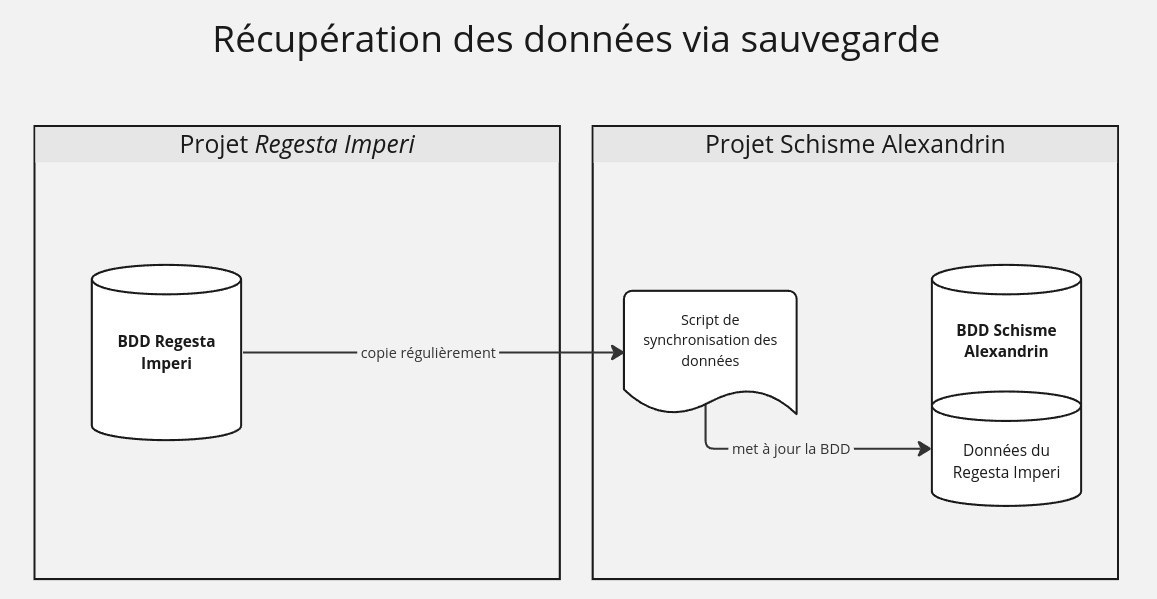
\includegraphics[width=10cm]{images/recup-donnees-sauvegarde.jpg}
    %légende
    \caption{Schéma représentant la récupération des données manuellement}
    %label
    \label{fig:schemadonneessauvegarde}
\end{figure}


    \subsection{Cas des données récupérées grâce à une API}

En récupérant les donnés à partir d'une API, nous nous assurons de toujours récupéré les données à jour. Par ailleurs, cette solution est plus facile car il est juste nécessaire de se connecter à l'API du projet. Mais le risque repose sur le fait que si le projet est abandonné ou plus maintenu, nous risquons de ne plus accéder aux données car l'API ne fonctionnera plus également.\\

\begin{figure}[H]
%centrer l'image
    \centering
    %commande qui permet de charger une image
    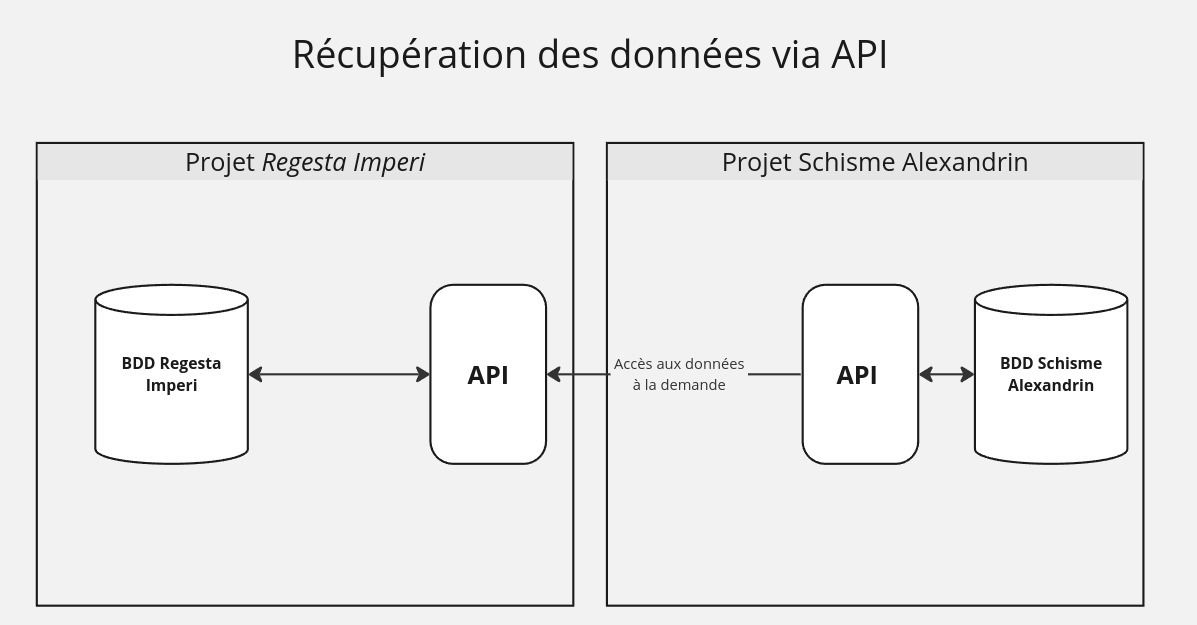
\includegraphics[width=10cm]{images/recup-donnees-api.jpg}
    %légende
    \caption{Schéma représentant la récupération des données grâce à une API}
    %label
    \label{fig:schemaAPI}
\end{figure}

    \subsection{Cas des données récupérées grâce à une API et une sauvegarde des données}

Ce dernier cas de figure présente une solution idéale, puisqu'elle consiste à récupérer les données à la fois grâce à l'API et en téléchargeant les données. Cela permet de s'assurer d'avoir toujours accès aux données à jour en ayant à la fois une connexion à l'API et un script de synchronisation de données. Par ailleurs, si le RI Online n'est plus maintenu, on est assuré d'avoir les données au sein du projet. En revanche, cette solution est plutôt coûteuse à mettre en place et à maintenir.\\

\begin{figure}[H]
%centrer l'image
    \centering
    %commande qui permet de charger une image
    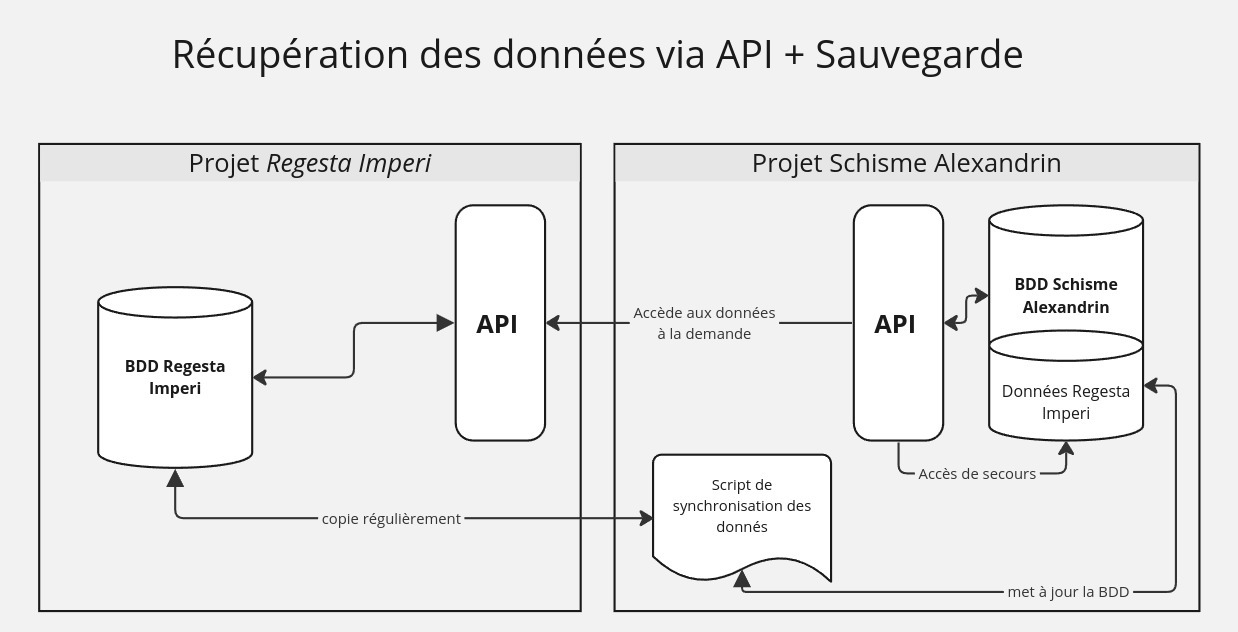
\includegraphics[width=10cm]{images/recup-donnees-api-and-backup.jpg}
    %légende
    \caption{Schéma représentant la récupération des données manuellement et grâce à une API}
    %label
    \label{fig:schemaAPIetbackup}
\end{figure}





La modélisation de données a permis de mettre en lumière plusieurs enjeux concernant le projet du schisme Alexandrin. Tout d’abord, le contexte historique dépeint de nombreux faits et acteurs rassemblés dans un corpus documentaire très vaste, estimé à environ 11.000 documents à terme. Ensuite, l’analyse de divers projets d’humanités numériques nous a permis d’évaluer les modèles de données et technologies à envisager. Les chercheurs de Aachen veulent s’inspirer des entrées du papsturkunden et du Regesta Pontificum Romanorum, et utiliser le schéma XML CEI. Enfin, s’atteler à la récupération de ces données peut s'avérer complexe :  celles-ci sont éparpillées entre plusieurs projets, sous différents formats et accessibles de manière non-uniforme. Actuellement, le premier objectif de ce projet est d’accéder au Jaffé 2 grâce à l’OCR, afin de pouvoir faciliter la recherche textuelle, et à terme pouvoir le traduire en anglais. Il est également important de noter que pour le moment, seulement les données du RI Online sont accessibles, et seraient ainsi les premières à être intégrées au projet.